\documentclass[sn-mathphys,iicol]{sn-jnl}% Math and Physical Sciences Reference Style 
%\documentclass[default,iicol]{sn-jnl}% Default with double column layout      

\jyear{2022}%

\raggedbottom
%%\unnumbered% uncomment this for unnumbered level heads

\usepackage{verbatim}
\usepackage{graphicx}

\usepackage{xspace}
\newcommand{\FC}       {Freechains\xspace}
\newcommand{\reps}     {\emph{reps}\xspace}
\newcommand{\onerep}   {\emph{1~rep}\xspace}
\newcommand{\nreps}[1] {\emph{#1~reps\xspace}}
\newcommand{\code}[1]  {\texttt{\small{#1}}}
\newcommand{\Xon} {$1{\rightarrow}N$\xspace}
\newcommand{\Xno} {$1{\leftarrow}N$\xspace}
\newcommand{\Xnn} {$N{\leftrightarrow}N$\xspace}
\newcommand{\Xoo} {$1{\leftrightarrow}1$\xspace}
\newcommand{\Xo}  {$1{\hookleftarrow}$\xspace}
\newcommand{\lin}[1]{(\emph{ln. #1}\xspace)}
\newcommand{\linx}[1]{\emph{ln. #1}\xspace}

\renewcommand{\theenumi}{\alph{enumi}}

\hyphenation{off-line}

\begin{document}

\title[Article Title]{
    Symmetric Peer-to-Peer Applications
}

\author{\fnm{Francisco} \sur{Sant'Anna} \email{francisco@ime.uerj.br}}
\affil{\orgdiv{Department of Computer Science}, \orgname{Rio de Janeiro State University}, \orgaddress{\country{Brazil}}}

\abstract{
In real-time networked applications, such as collaborative documents, users can
interact remotely and yet share the exact same experience as if they were using
a single machine.
%
In this work, we propose a middleware for \emph{symmetric peer-to-peer
applications} in which decentralized instances can broadcast asynchronous
events and yet conform to identical behavior.
%
Peers are allowed to join and leave the network at any time.
Application developers must adhere to a deterministic and stateless API.
%, and only supports pre-allocated memory.
%
The middleware is responsible for synchronizing the events in a global shared
timeline across the network.
Also, based on memory snapshots and deterministic simulation, a ``time machine''
can rollback conflicting peers to resynchronize their states.
%
We show that the middleware can handle applications with over 20 peers in a
heterogeneous topologies under high churns.
For instance, in a simulation scenario with a network latency of 50ms and 25
events per minute, the peers need to roll back and resynchronize only 3\% of
the time.
}

\keywords{
collaboration, determinism, peer-to-peer, time machine
}

%%\pacs[JEL Classification]{D8, H51}

%%\pacs[MSC Classification]{35A01, 65L10, 65L12, 65L20, 65L70}

\maketitle

\section{Introduction}
\label{sec.introduction}

Real-time networked applications allow multiple users to interact remotely and
yet share the same experience.
Examples of these \emph{symmetric distributed applications}~\cite{gals} are
collaborative documents, watch parties, and multi-player games.
%~\cite{TODO:collab}.
%
In order to reproduce the exact behavior in multiple devices, the application
must be able to synchronize time and execution across the network.
In addition, since users can interact asynchronously with the application,
event occurrences must somehow be synchronized back across devices.

A common approach towards symmetric applications is to introduce a middleware
to orchestrate events and time in the network~\cite{gals,croquet}.
This way, applications developers can rely on middleware primitives to trigger
events, which are intercepted and synchronized in a global shared timeline
across the network.
Developers must also restrict themselves to deterministic and stateless calls
only, such that execution can be equally reproduced in all nodes according to
the shared timeline. %~\cite{TODO:det_reprod}.
However, current solutions depend on a central server to interconnect network
nodes and determine a shared timeline.

In this work, we propose \emph{symmetric peer-to-peer applications}, which
do not rely on central servers for coordination.
Peers in the application form a dynamic network graph and communicate only
with direct neighbours, as in typical unstructured peer-to-peer
networks~\cite{p2p.survey}.
Events are flooded in the graph and are applied with a small deadline delay to
compensate the network latency.
To deal with events received out of order or too late, a distributed time
machine can rollback peers to a previous state and reapply events in order and
in time.
Our main contribution is the design of a middleware to ensure that all peers
    (a) meet event deadlines,
    (b) advance in sync in real time, and
    (c) can leave and join the network and remain symmetric.

We perform simulations with over 20 peers in a 5-hop mixed topology with cycles
and straight lines.
We vary the network latency and peer churn, as well as the frequency and
deadlines of events.
%
We then measure (a) the recurrence of time travels, (b) the real-time pace of
peers, and (c) the recoverability from churns, such that they validate our
goals above, respectively.
%
As results, we show that the last two goals are met even under extreme
conditions: peers exhibit a time mismatch of under $0.2\%$ and take less than
$1.5s$ to recover from churns.
%
For the first goal, we analyze the scenarios in which the middleware can meet
event deadlines with the desired performance.
As an example, peers need to roll back only $3\%$ of the time under a scenario
with a network latency of $50ms$ and 25 events per minute.

In Section~\ref{sec.related}, we revisit existing solutions for symmetric
distributed applications.
In Section~\ref{sec.tml}, we detail the architecture of our middleware, its
programming API, and how it orchestrates peers.
%In Section~\ref{sec.app}, ...
In Section~\ref{sec.eval}, we evaluate our design under a number of scenarios.
In Section~\ref{sec.conclusion}, we conclude this work.

\section{Related Work}
\label{sec.related}

% docs.google.com/spreadsheets/d/1CpMmEgabJq2XQeTDW_BNCV4JWrcMlELuaEjDtw7kwg0/
\begin{figure}
  \centering
  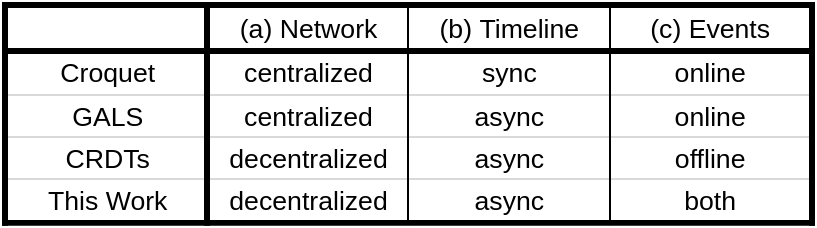
\includegraphics[width=\linewidth]{table}
  \caption{
    Related work regarding
        (a) how the network is organized,
        (b) how global time is determined, and
        (c) how events are broadcast and applied.
    \label{fig.table}
  }
\end{figure}

\begin{figure*}
  \centering
  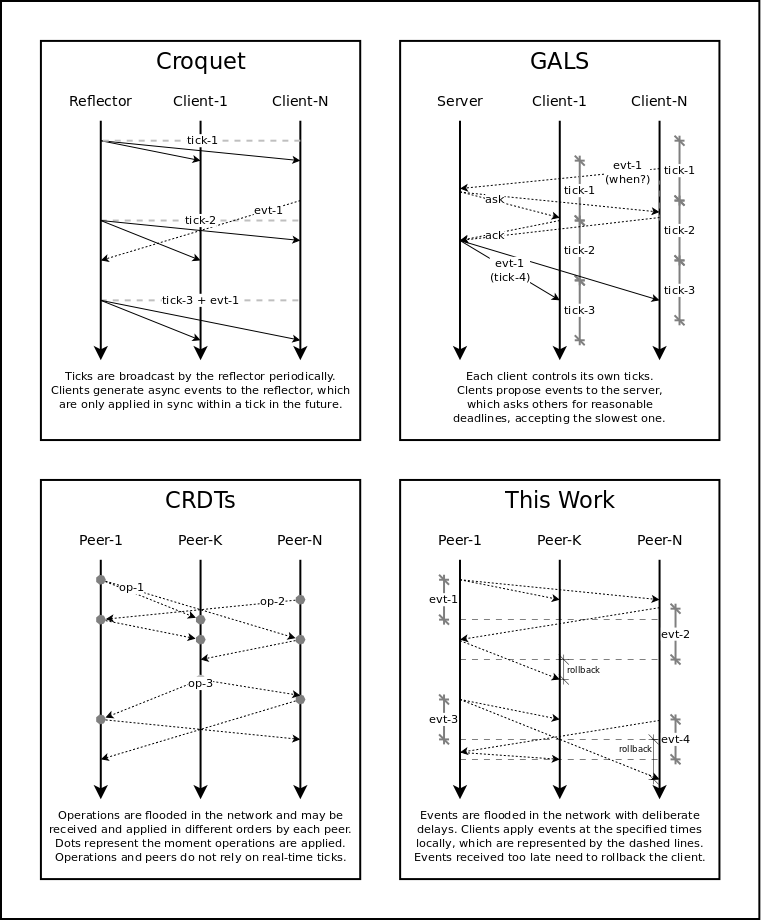
\includegraphics[width=\linewidth]{algos}
  \caption{
    \label{fig.algos}
    Four approaches to symmetric distributed applications: Croquet, GALS,
    CRDTs, and this work.
    The vertical arrows in parallel represent the timelines in nodes in the
    network.
    The arrows crossing nodes represent communication between them.
  }
\end{figure*}

In this section, we revisit existing solutions for symmetric distributed
applications.
We focus on
    (a) how the network is organized,
    (b) how global time is determined, and
    (c) how events are propagated and applied.
Figure~\ref{fig.table} compares three selected works regarding these aspects.

Croquet~\cite{croquet,croquet.site} guarantees bit-identical real-time behavior
for users in collaborative distributed environments.
%
As detailed in Figure~\ref{fig.algos}, a centralized \emph{reflector} issues
periodic ticks, such that all nodes in the network advance together according
to a synchronized global shared clock.
If a user generates an event, it is sent back to the reflector, which
broadcasts the event in the next tick, which all nodes apply in sync.
%
Croquet takes periodic snapshots of the whole application state in order to
support late joins to a running session.
The new node just needs to request the latest snapshot and simulate the
remaining events to reach the current running state.
%
As indicated in Figure~\ref{fig.table}, Croquet relies on a centralized
network (a), in which nodes advance in sync (b), and in which event broadcasts
and outcomes depend on the central server to be online (c).

GALS~\cite{gals} shares the same goals with Croquet, but with some tradeoffs,
mostly favoring clients with slow connections.
As detailed in Figure~\ref{fig.algos}, instead of advancing ticks in sync with
the server, clients have their own independent local clocks.
Event generation requires two round trips (\emph{when→ask→ack→tick}), resulting
in dynamic deadlines according to the slowest client.
%
On the one hand, ticks do not generate any traffic, and clients experience
smooth frame transitions, even those with poor connections.
On the other hand, events take longer to apply and clients may experience
occasional freezes.
The syncing protocol also requires extra bookkeeping to deal with clock drifts
and client disconnections~\cite{gals}.
%
As indicated in Figure~\ref{fig.table}, GALS also relies on a centralized
network (a), but in which nodes advance time independently (b), and in which
event broadcasts and outcomes still depend on the central server to be online
(c).

In both solutions, the network advances together in real time as a whole, with
a total order among events, which is determined by a central server that must
be permanently online.
All clients compute events in sequence, respecting timestamps, and using only
deterministic and stateless calls.
This way, it is guaranteed that all clients reach the same state, and
observe bit-identical steps.

An antagonistic approach to deterministic reactions to events is to model the
applications with Conflict-free Replicated Data Types~\cite{crdts}.
CRDTs are designed in such a way that all operations are commutative, so that
the order in which they are applied does not affect the final outcome.
%
As detailed in Figure~\ref{fig.algos}, peers can communicate operations
directly to each other with no central authority.
Also, since operations need not to be ordered, they can be applied at the
very first moment they are generated or received, even if the originating peers
are offline.
%
Note that it is not possible to timestamp commutative operations under a unique
global shared clock.
Hence, there is no notion of a timeline in which peers go through bit-identical
steps, but they do eventually reach the same state~\cite{crdts.eventual}.
%
On the one hand, the main advantage of CRDTs is to support local-first
software~\cite{local}, since they can work offline in the same way as online.
On the other hand, they provide very restrictive APIs (the CRDTs themselves),
and do not support real-time consensus among peers~\cite{crdts.consensus}.
%
As indicated in Figure~\ref{fig.table}, CRDTs work on decentralized networks
(a), in which peers advance independently (b), and in which operations can be
applied immediately, even while offline (c).
%
Automerge along with its accompanying Hypermerge peer-to-peer infrastructure
is an example of decentralized CRDTs~\cite{p2p.automerge,p2p.pushpin}.

In this work, as indicated in Figure~\ref{fig.table}, our goal is to support
peer-to-peer (a) real-time symmetric execution, while still tolerating
out-of-order (b) and offline (c) event generation.
%
As detailed in Figure~\ref{fig.algos}, peers have independent timelines and
can communicate events directly to each other.
Event deadlines are delayed to be able to reach other peers in time.
In the case a deadline is missed, the peer rolls back in time and then fast
forwards execution until it catches real-time behavior again.
%
Like Croquet and GALS, peers compute events in sequence using deterministic and
stateless calls only.

We now discuss related work on time machines.
%
Regarding decentralized solutions, Fusion~\cite{fusion} is a state
synchronization networking library for the Unity game engine.
It provides networked tick-based simulation in two modes: client-server
(\emph{hosted mode}) and peer-to-peer (\emph{shared mode}).
The hosted mode is based on continuous memory snapshots, which allows for
full rollbacks when clients diverge.
However, the shared mode is less powerful and only supports eventual
consistency among clients.
We presume that continuous memory snapshots would be too costly without a
central server.
%
Regarding single-user local machines, the video game Braid%
\footnote{Braid: \url{http://braid-game.com/}}
is designed on the assumption that players have unrestricted rollbacks as part
of the game mechanics.
Like Fusion, the implementation is based on continuous memory snapshots,
instead of deterministic simulation as we propose in this work.
%
Schuster~\cite{tml.js} proposes a simple API for time travelling in
event-driven JavaScript:
    \code{init()} to return an initial state;
    \code{handle(evt,mem)} to process events and modify state; and
    \code{render(mem)} to output the current state.
As we describe next, we use a similar approach by separating state mutation
from rendering~\cite{tml.alive}.

\section{The Middleware \& Programming API}
\label{sec.tml}

Our middleware is written in C and relies on the library \emph{SDL}%
\footnote{SDL: \url{http://www.libsdl.org}}
to deal with the network, timers, and input events, such as mouse clicks and
key presses.
The full source code%
\footnote{Code: \url{http://github.com/TODO-hidden-blind-review}}
is under 500 lines of code.

\begin{figure}
    \centering
    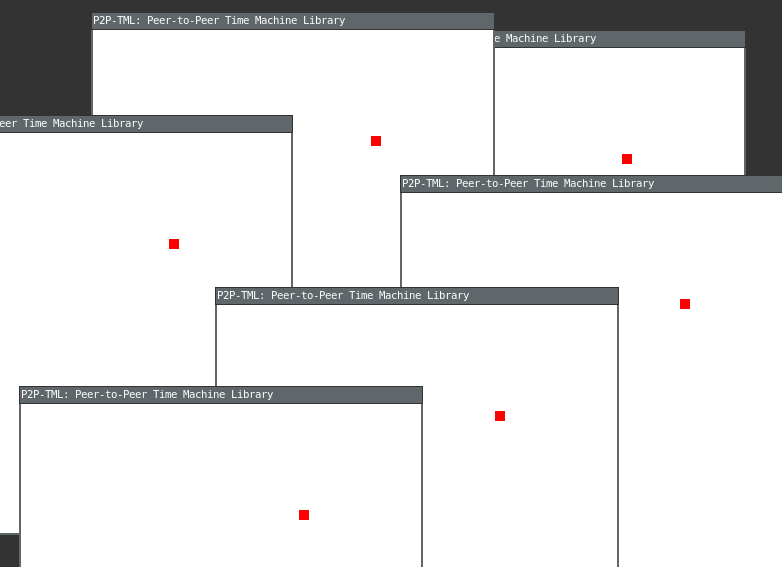
\includegraphics[width=\linewidth]{move}
    \caption[XXX] {
        A moving rectangle is controlled by peers connected indirectly.
        Users can press \code{↑ ↓ → ←} to change the direction of the
        rectangle or \code{SPACE} to pause the application.
        The inputs are applied simultaneously in all peers, as if they were
        mirrors of a single application.
        Video: \url{http://youtube.com/TODO-hidden-blind-review}
        \label{fig.move}
    }
\end{figure}

We guide our discussion through the didactic example of Figure~\ref{fig.move},
in which multiple users control the direction of a moving rectangle using the
arrow keys.
The six instances are connected in a peer-to-peer network, such that most
peers can only communicate indirectly to each other.
%
The application is symmetric in the sense that if any user presses a key, a
corresponding event is broadcast and applied in all peers simultaneously, as
if they were a single mirrored machine.
At any moment, if a user pauses the application, all peers are guaranteed to
pause exactly at the same frame, with the rectangle ``bit-identically'' at the
very same position.

\begin{figure}
  \centering
  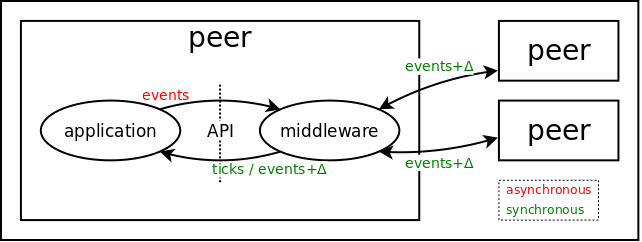
\includegraphics[width=\linewidth]{middleware}
  \caption{
    Applications generate asynchronous events and communicate through an API
    with the middleware.
    The middleware orchestrates the peers, synchronizing their ticks locally
    and broadcasting events with a deadline delay ($\Delta$).
    \label{fig.middleware}
  }
\end{figure}

In Figure~\ref{fig.middleware}, a peer is depicted as an application that uses
an API to communicate with the middleware.
The application itself is not aware of the network and has no direct access to
other peers, which communicate transparently through the middleware.
The application generates asynchronous events that go through the middleware,
which synchronizes them with a timestamp with a deadline delay ($\Delta$)
scheduled to the future, such that all peers can satisfy.
The middleware controls the execution of the application by issuing ticks and
synchronized events.
Note that ticks need not to be broadcast, only $\Delta$ events.

The main job of the middleware is to deal with the uncertainties of the
network in order to preserve the symmetric behavior across peers.
As described in the Introduction, the middleware ensures that all peers
    (a) meet event deadlines,
    (b) advance in sync in real time, and
    (c) can leave and join the network and remain symmetric:
%
\begin{enumerate}
\item \textbf{Event Deadlines:}
Due to the inherent latency of networks, peers generate events with a
deliberate $\Delta$ so that they can reach other peers in time to be applied in
sync.
%We first assume a predetermined delay for the sake of simplicity.
Nevertheless, a peer ahead of time may receive an event that should have been
applied in the past. %, even considering its $\Delta$.
In this case, the middleware automatically rolls back the peer, applies the
event at the correct time, and then fast forwards the peer, re-applying all
remaining events up to the real time.
As we detail further, rolling back a peer requires to simulate the whole
application execution and event occurrences from the beginning.
As an optimization, the middleware takes periodic snapshots locally to avoid
full simulation.
%
\item \textbf{Time Synchronization:}
Since peers run in different machines, their timelines will inevitably be out
of sync because applications are launched locally at different times, and
because internal clocks may diverge over time (e.g., from rollbacks or timer
polling inaccuracies).
The middleware assumes the maximum time among all peers the be the
``correct real time'', so that other peers must fast forward to catch up with
it.
Therefore, in order to determine the maximum time and synchronize the clocks,
the middleware proceeds as follows:
    (a) peers broadcast \code{SYNC} events periodically with their local
        times, and
    (b) if a peer is behind a received \code{SYNC}, it advances its frames
        proportionally faster to catch up in time.
%
To avoid abrupt visual changes, the middleware makes smooth time transitions
that take up to $1s$ to complete.
%
\item \textbf{Peer Churn:}
Considering that we target dynamic peer-to-peer networks, it is important that
the middleware can handle arrival and departure of peers seamlessly.
Note that high churn may lead to intermittent network partitions.
Given our unstructured approach, nothing needs to be done when a peer leaves
the network.
However, when a peer joins the network, the middleware needs to ensure that it
receives from other peer all events that ever happened, in order.
This is trivial since all peers already need to hold the full event history (as
described in item (a)).
% including their absolute timestamps in the shared timeline.
\end{enumerate}

\subsection{The Programming API}
\label{sec.tml.api}

The middleware expects to take full control of the application execution in
order to manipulate its timeline and disseminate events in the network.
For this reason, the basic programming API is to call a \code{loop} function
passing a set of callbacks, which the middleware uses to communicate with the
application:

{\footnotesize
~
\begin{verbatim}
int main (void) {
    p2p_loop (
        1,              // peer identifier
        50,             // simulation FPS
        sizeof(G), &G,  // pre-allocated full state
        cb_ini,         // init/quit callback
        cb_sim,         // simulation callback
        cb_ren,         // rendering callback
        cb_evt          // events callback
    );
}
\end{verbatim}
~
}

The middleware assumes that each peer assigns itself a unique identifier (e.g.,
a combination its MAC \& IP addresses).
%, such as TODO~\cite{TODO:hash}.
The FPS must be the same in all peers to ensure bit-identical simulation.

Note that the use of callbacks is a common technique for event-driven
programming in Games, GUIs, and interactive applications in general, sharing
recognition with related techniques such as \emph{MVC},
\emph{Publish-Subscribe}, and \emph{Observer} patterns~\cite{meyer,nystrom}.
%
Furthermore, the default run-to-completion semantics of callbacks is key to
ensure the desired determinism, since unlike threads, they run sequentially and
atomically from start to end~\cite{events,threads}.

%As pointed by Berry and Benveniste, the advantages of deterministic systems should
%be obvious: there is no reason a programmer should want his/hers
%programs to behave in some non-deterministic manner [2].
%A. Benveniste and G. Berry. The Synchronous Approach to Reactive and Real-
%Time Systems. Proceedings of the IEEE, 79(9):1270–1282, 1991.
%see also twelve

\subsubsection{Application State}
\label{sec.tml.api.state}

The variable \code{G} passed to the middleware holds the full application
state.
This allows the middleware to take memory snapshots and rollback to previous
states.
In our guiding example of Figure~\ref{fig.move}, the application only needs to
hold the rectangle position and direction:

{\footnotesize
~
\begin{verbatim}
struct {
    int x,  y;   // position
    int dx, dy;  // direction speed
} G;
\end{verbatim}
~
}

If dynamic allocation is required, it is necessary to hold a finite memory
pool in \code{G} with a custom allocator.
This is a limitation of C, since languages with serialization and
meta-programming offer better mechanisms to take memory snapshots.
Another alternative is to provide a serialization callback, which we left for
future work.

\subsubsection{Application Events}
\label{sec.tml.api.events}

When an application generates events, they need to be broadcast to the network
so that all peers behave the same.
Note that application events may (or may not) differ from low-level local
system events.
%which may or may not be mapped 1-to-1 in the callback \code{cb\_evt}.
%
The middleware predefines three events for all applications:
    \code{P2P\_EVT\_SYNC} represents synchronization events
        (Section \ref{sec.tml}.b).
    \code{P2P\_EVT\_START} represents the beginning of the simulation, and
    \code{P2P\_EVT\_TICK} is generated every frame.
The other application-specific events must be declared by the programmer in an
enumeration.
In our example, we define a new event \code{P2P\_EVT\_KEY} to represent key
presses:

{\footnotesize
~
\begin{verbatim}
enum {
    P2P_EVT_KEY = P2P_EVT_NEXT // key is next to predefs
};
\end{verbatim}
~
}

\subsubsection{Initialization Callback}
\label{sec.tml.api.cb_ini}

The middleware calls \code{cb\_ini} twice: at the beginning and at the end of
the loop.
The callback should initialize (and finalize) the network topology, as well as
static immutable globals that can live outside the simulation memory, such as
the window and image textures in our example:

{\footnotesize
~
\begin{verbatim}
void cb_ini (int ini) {
    if (ini) {
        <...> // create the SDL window
        <...> // open the arrow PNG images
        // create peer links (peer-id, ip, port)
        p2p_link(2, "192.168.1.2", 5000);
    } else {
        <...> // destroy the SDL window
        <...> // destroy the arrow PNG images
        // destroy peer links
        p2p_unlink(2);
    }
}
\end{verbatim}
~
}

\subsubsection{Simulation Callback}
\label{sec.tml.api.cb_sim}

The middleware calls \code{cb\_sim} every frame or event occurrence, which
should affect the simulation state \code{G} deterministically.
Occurring events are passed as arguments to the callback, which must never
perform any side effects, such as stateful calls or rendering frames.
In our example, we modify the state of the rectangle as follows:
    on \code{START}, reset its position and speed;
    on \code{TICK},  increment its position based on the current speed; and
    on \code{KEY},   modify its speed:

{\footnotesize
~
\begin{verbatim}
void cb_sim (p2p_evt evt) {
    switch (evt.id) {
        case P2P_EVT_START: // resets pos and speed
            G.x = G.y = G.dx = G.dy = 0;
            break;
        case P2P_EVT_TICK:  // increases position
            G.x += G.dx * VEL;
            G.y += G.dy * VEL;
            break;
        case P2P_EVT_KEY:   // modifies speed
            switch (evt.pay.i1) {
                case SDLK_UP:
                    G.dx = 0;
                    G.dy = -1;
                    break;
                <...> // similar for other keys
            }
            break;
    }
}
\end{verbatim}
~
}

The calls to \code{cb\_sim} normally happen during real-time simulation, i.e.,
while the user is interacting with the application.
However, if the peer is out of sync, the middleware may ``time travel'' and
call the simulation many times to go back and forth and catch up with real
time.
This is the reason why we define \code{START} as an event like any other:
travelling requires to simulate the execution from the beginning, event by
event.

\subsubsection{Rendering Callback}
\label{sec.tml.api.cb_ren}

Time travelling is also the reason why \code{cb\_sim} must be separated from
the rendering callback \code{cb\_ren}~\cite{tml.js}, which would otherwise
render the screen multiple times while travelling.
The middleware renders the screen after each frame in real time.
%, which the middleware calls only on real-time frames.
In our example, \code{cb\_ren} just needs to redraw the rectangle at the
current position:

{\footnotesize
~
\begin{verbatim}
void cb_ren (void) {
    <...> // clears the SDL window
    // redraws the rectangle at the current position
    SDL_Rect r = { G.x, G.y, 20, 20 };
    SDL_DrawRect(&r);
}
\end{verbatim}
~
}

\subsubsection{Events Callback}
\label{sec.tml.api.cb_evt}

The callback \code{cb\_evt} is called by the middleware in real time, whenever
a local SDL event occurs.
This callback has two goals:
    (a) map and broadcast application events, and
    (b) provide instant feedback to the user.
%As mentioned previously,
Not all local low-level events need to broadcast application events in the
network.
The callback is allowed to perform side effects, such as modifying the network
topology, or exhibiting instant feedback on the screen.
In our example, we only generate application events for the 5 key events of
interest, but we also exhibit the pressed key in real time as a visual
feedback:

{\footnotesize
~
\begin{verbatim}
int cb_evt (SDL_Event* sdl, p2p_evt* evt) {
    if (sdl->type == SDL_KEYDOWN) {
        if (sdl->key == <any-of-the-keys>) {
            SDL_DrawImage(<img-of-the-key>);
            *evt = (p2p_evt){ P2P_EVT_KEY,sdl->key };
            return 1; // generate application event
        }
    }
    return 0; // otherwise, do not generate any event
}
\end{verbatim}
~
}

\subsection{Middleware Orchestration}
\label{sec.tml.middleware}

We now detail how the middleware orchestrates an application and ensures that
all peers
    (a) meet event deadlines,
    (b) advance in sync in real time, and
    (c) can leave and join the network and remain symmetric.

\subsubsection{Event Broadcasting}
\label{sec.tml.middleware.events}

As illustrated in Figure~\ref{fig.middleware}, events are broadcast between
peers with a deadline $\Delta$ scheduled to the future, such that all peers are
able to apply them in sync.
%
To prevent broadcast cycles, each peer keeps a collection of the highest
timestamps it received from each other peer, such that lower numbers can be
ignored when received.
Since we rely on TCP connections, it is not possible to receive out-of-order
timestamps attached to a given source peer.
When the middleware receives a higher number from a given peer, it updates this
number and triggers a broadcast to neighbours.
%
%As mentioned in Section~\ref{sec.tml.api}, we assume that peers assign
%themselves unique identifiers in a contiguous range, such that they fit in a
%simple vector of timestamps.
%Therefore, this is not a severe limitation, and a separate mechanism could be
%used for assignments, with few modifications to the core of the middleware.

When receiving an unseen event, the middleware also enqueues it in timestamp
order and calls the application callback \code{cb\_sim} at the appropriate
time.
Peers must keep the full event queue in memory for two reasons:
    (a) receiving a late event may reorder it and require a time travel, and
    (b) peers that join the network need to receive all events.
%
Therefore, the middleware keeps a queue of ``packets'', which includes the
event and additional metadata:

{\footnotesize
~
\begin{verbatim}
typedef struct {
    uint8_t  src;       // source peer
    uint32_t tick;      // tick to apply
    p2p_evt  evt;       // event id + payload
} p2p_pak;

struct {
    int i;  // next event to apply in real time
    int n;  // number of events in the queue
    p2p_pak buf[MAX];   // queue of packets
} PAKS;
\end{verbatim}
~
}

\subsubsection{The Main Loop}
\label{sec.tml.middleware.loop}

The middleware main loop \code{p2p\_loop} is responsible for calling the
application callbacks, and also controlling its timeline.
The loop continuously checks for network packets, local inputs, and time ticks,
as follows:

{\footnotesize
~
\begin{verbatim}
01  void p2p_loop (...,cb_ini,cb_sim,cb_ren,cb_evt) {
02    cb_ini(1);    // initialization
03    cb_sim(<P2P_EVT_START>);
04
05    while (<app-running>) {
06      if (<next-network-packet>) {
07        // fast forward if I'm late
08        if (<packet-sync-future>) {
09          p2p_travel(<now>, <pak-sync-time>, <vel>);
10        }
11
12        // travel back & forth if I'm early
13        if (<packet-evt-past>) {
14          p2p_travel(<now>, <pak-evt-time>, <vel>);
15          p2p_travel(<pak-evt-time>, <now>, <vel>);
16        }
17
18        // real time if I'm on time
19        if (<packet-evt-ok>) {
20          cb_sim(<packet-evt>);
21          cb_ren();
22        }
23      }
24
25      if (<next-local-input>) {
26        // broadcast local event
27        p2p_evt evt;
28        if (cb_evt(&evt)) {
29          p2p_bcast(<future>, &evt);
30        }
31      }
32
33      // simulate tick in real time
34      if (<next-local-tick>) {
35        cb_sim(<P2P_EVT_TICK>);
36        <application-snapshot-every-second>
37        cb_ren();
38      }
39    }
40
41    cb_ini(0);    // finalization
42  }
\end{verbatim}
~
}

The function receives the application callbacks as arguments \lin{1}.
%(Section~\ref{sec.tml.api}).
We first (and last) call \code{cb\_ini} to initialize (and finalize) the
application \lin{2,41}.
Then, we call \code{cb\_sim} \lin{3}, passing the event \code{START} to start
the application in real time.
%(Sections~\ref{sec.tml.api.events}~and~\ref{sec.tml.api.cb_sim}).
The main loop \lin{5--39} checks continuously for network packets \lin{6--23},
local input events \lin{25--31}, and time ticks \lin{33--38}.

Regarding network packets, if we receive a time synchronization packet
\code{SYNC} from the future \lin{7--10}, then we fast forward the application
to catch up in time. % (Section~\ref{sec.tml}.b).
If we receive an event that should have been applied in the past \lin{12--16},
then we travel back and forth. % (Section~\ref{sec.tml}.a).
Otherwise, we just apply the event in real time \lin{18--22}.
%(Section~\ref{sec.tml.api.cb_sim}).
We detail the function \code{p2p\_travel} in
Section~\ref{sec.tml.middleware.travel}.
%
Regarding local inputs, we call \code{cb\_evt} to signal if the event should be
broadcast \lin{26--30}, and transformed into an application event.
%(Section~\ref{sec.tml.api.cb_evt}).
%
Regarding time ticks, we call \code{cb\_sim} and \code{cb\_ren} in real time
\lin{33--38}.
The middleware also takes periodic snapshots of the application state to
optimize time travelling. % (Section~\ref{sec.tml.api.state}).

\subsubsection{The Time Machine}
\label{sec.tml.middleware.travel}

The last important mechanism of the middleware is the time machine, which
allows to move the application back and forth in time:

{\footnotesize
~
\begin{verbatim}
01  void p2p_travel (int from, int to, int ms) {
02    for (i=from..to) {
03      int bef = <tick-of-snapshot-before-i>
04      <restore-snapshot-at-bef>
05      for (j=bef..i) {
06        cb_sim(<tick-or-evt-at-j>)
07      }
08      cb_ren();
09      <delay-ms>
10    }
11  }
\end{verbatim}
~
}

The function \code{p2p\_travel} time travels the application, starting at tick
\code{from}, tick by tick \lin{2--10}, until it reaches tick \code{to}.
The loop can travel in both directions, i.e., \code{from} may be higher than
\code{to}.
At each step, we need to find the tick \code{bef} with the closest past
snapshot \lin{3}, restore it \lin{4}, and than simulate the remaining steps
from the snapshot to the desired tick \lin{5--7}.
We also exhibit each step with a small \code{ms} delay \lin{8--9} so that users
experience smooth time transitions.

\subsubsection{Summary}
\label{sec.tml.middleware.summary}

This section provides an overview of the middleware implementation to answer
how it ensures the desired properties in concrete terms as follows:
    (a) peers meet event deadlines either travelling back and forth or in real
        time (Section \ref{sec.tml.middleware.loop}: \linx{12--16} or
        \linx{18--22});
    (b) peers synchronize their clocks with periodic \code{SYNC} packets that
        fast forward late peers (Section \ref{sec.tml.middleware.loop}:
        \linx{7--10}); and
    (c) peers can join the network at any time and still catch up in time by
        receiving the full event history
        (Section~\ref{sec.tml.middleware.events}).

%\newpage
\section{Evaluation}
\label{sec.eval}

In this section, we evaluate if our design meets the goals to ensure that all
peers
    (a) meet event deadlines,
    (b) advance in sync in real time, and
    (c) can leave and join the network and remain symmetric.
%
We perform simulations varying the network latency and peer churn, as well as
the frequency and deadlines of events.
%
We then measure
    (a) the recurrence of time travels,
    (b) the real-time pace of peers, and
    (c) the recoverability from churns,
such that they validate our goals above, respectively.

Regarding (a), if a peer experiences a time travel, it means that it received
an event after its deadline.
We then count all time travel occurrences in our evaluation.
%
Regarding (b), we use an absolute simulation clock to track, in real time, the
execution pace of each peer.
% in comparison to the reference peer, which is the one most advanced in time.
We then count the mismatches between the clocks in our evaluation.
%
Regarding (c), we make peers leave and join the network periodically, possibly
creating partitions.
We then assert that they all catch up in real time within a short period in our
evaluation.

\begin{figure*}
  \centering
  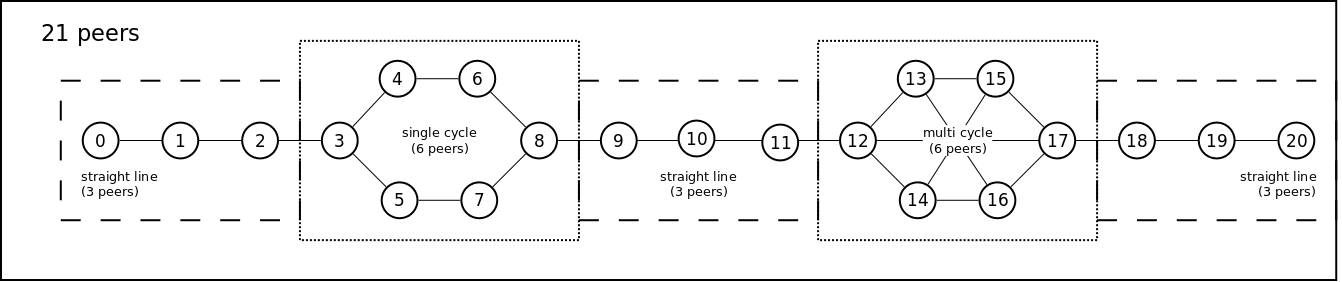
\includegraphics[width=\linewidth]{topo}
  \caption{
    \label{fig.topo}
    Network topology: 21 peers organized as a straight line ($0-3$), a simple
    cycle ($3-8$), a second straight line ($8-11$), a full connected cycle
    ($12-17$), and a third straight line ($17-20$).
    %An optional link ($0,20$) creates a long cycle in the network.
  }
\end{figure*}

\begin{figure}
  \centering
  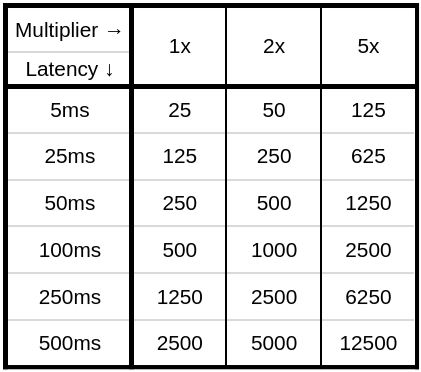
\includegraphics[width=2in]{mult}
  \caption{
    \label{fig.mult}
Event $\Delta$s in $ms$ considering the network latency, deadline multiplier,
and the average of 5 hops between peers from Figure~\ref{fig.topo}.
    }
\end{figure}

We perform simulations with 21 peers using the mixed topology of
Figure~\ref{fig.topo}, with peers organized in straight lines and cycles.
The topology has an average of 5 hops between peers (e.g., \code{4-16} are 7
hops away).
%
We run the application main loop at $50~FPS$ ($20ms$ per frame) and calculate
the middleware overhead at each iteration.
We found a negligible overhead of $9us$ in the average, which corresponds to
less than $1/2000$ of the CPU time.
%
In order to have an absolute clock, we use a single machine to simulate all
peers, allowing us to merge their logs into a single file with a comparable
shared timeline.
%
We use \emph{NetEm}~\cite{netem} to simulate the network latency with a normal
distribution.
% (e.g., \code{tc qdisc add dev lo root netem delay 200ms 40ms distribution normal}).
%
We vary
    (i)   the network latency ($5-500ms$ between each peer),
    (ii)  the rate of events ($5-200~evt/sec$), and
    (iii) the deadline $\Delta$ multiplier ($1-5x$).
%
Figure~\ref{fig.mult} shows the $\Delta$s considering the network latency and
chosen multiplier.
For instance, a $50ms$ latency with a $2x$ multiplier results in
$\Delta=500ms$, i.e., each event is triggered with this deadline delay to
compensate the given latency and fixed average of 5 hops
($5 \times 50 \times 2 = 500$).

All simulation variations result in $108$ combinations.
We executed each combination $3$ times for $5$ minutes each.
We also make some modifications to evaluate peer churn, which requires to
re-execute the simulation.
The experiments take around $40$ hours to complete.

% https://docs.google.com/spreadsheets/d/1xK5_wF9MoR-SmPGWVj0sGLrHxhpPBlLjVoS8U-Y7zTQ/edit#gid=63016757

\begin{figure*}
  \centering
  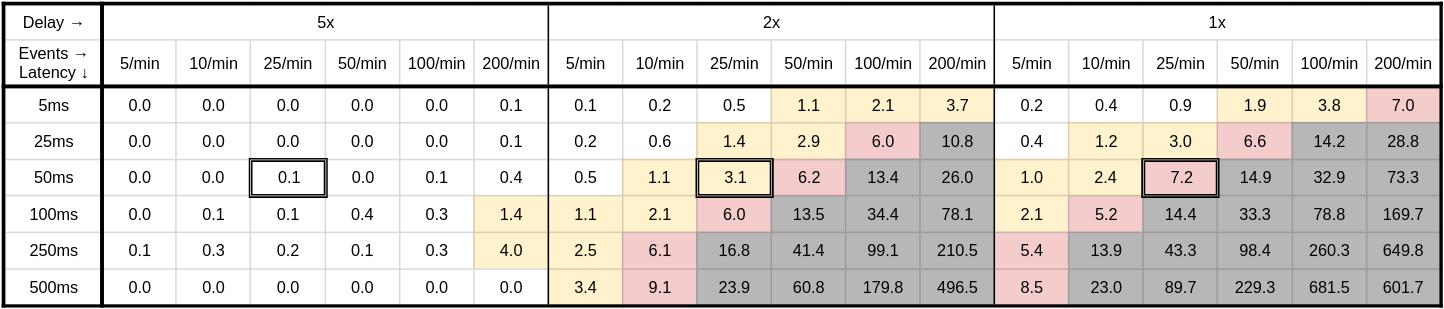
\includegraphics[width=\linewidth]{baks}
  \caption{
    \label{fig.baks}
The $5x$, $2x$, and $x$ $\Delta$ regions each contains $36$ measures for
multiple configurations of network latencies ($5-500ms$) and event rates
($5-200~evt/min$).
%
The color thresholds (\emph{white}, \emph{yellow}, \emph{red}, \emph{black})
are arbitrary but help to distinguish between regions of interest.
%
The experiments uses $1$ process for each peer in a single Linux machine
(\emph{Ubuntu 21.04, i7/16GB}).
    }
\end{figure*}

We now detail the results and how we instrument the middleware implementation
to measure the properties of interest above:

\textbf{(a) Recurrence of time travels:}
Every time a peer is ahead in time and needs to travel back, we output its id
and how much ticks it needs to travel back.
At the end, we measure the percentage of the sum of all time travel ticks over
the total simulation ticks.
As an example, if all peers sum $1000$ time travel ticks over $100k$
accumulated simulation ticks, then the final measure is $1\%$.
%
Figure~\ref{fig.baks} presents the results considering all combinations of
parameters (i), (ii), and (iii) above.
The colors indicate the feasibility of each tested scenario
    (\emph{white=good}, \emph{yellow=moderate}, \emph{red=poor},
    \emph{black=faulty}).
%
For instance, the three framed rectangles ($0.1$, $3.1$, and $7.2$) in the
figure represent the scenarios with $50ms$ network latency, generating
$25~evt/min$.
Each rectangle uses a different $\Delta$ multiplier, showing a good performance
for $5x$, moderate for $2x$, and poor for $1x$.

\textbf{(b) Real-time pace of peers:}
All peers output their ticks continuously, allowing us to compare them in the
shared timeline.
Every time we see a greater tick never seen in the timeline before, we start to
count smaller ticks from other peers, which constitute time violations.
As an example, if all peers sum $1000$ of such smaller ticks over $100k$
accumulated simulation ticks, then the final measure is $1\%$.
%
We also start each peer with a random delay of up to $10s$ to force a
synchronization mismatch at the beginning.
%
Considering all scenarios, the average is negligibly under $0.2\%$, with no
significant variance.
Therefore, we omit the resulting table (akin to Figure~\ref{fig.baks}), which
would not provide further insights.

\textbf{(c) Correctness of unstable peers:}
We tweak our simulation to make each peer remain $40s$ online and $20s$
offline in the average, including peers \code{9-11} in the middle of the
network.
This creates partitions in the network, which generate events out of sync that
require constant resynchronization between peers.
%
Then, to evaluate the network correctness under such high churn, we count how
much time a recovering peer takes to catch up in real time, as follows:
When a peer becomes online, we take the current maximum tick considering all
reachable peers, and then count the time the recovering peer takes to catch up.
We also assert that they all reach the same final state eventually.
%
Considering all scenarios, the average is $1.3$ seconds of recovering time,
with no significant variance.
Therefore, we also omit the resulting table (akin to Figure~\ref{fig.baks}).

\begin{comment}
$ vi test.c: // #define TEST_OFFLINE
$ sudo ./test-ana.sh 2>&1 | tee all.log
$ ./test-sheet.sh > sheet.log
$ ./test-sheet-2.sh > sheet-2.log
$ lua5.3 test-sheet-2.lua sheet-2.log > /tmp/x
$ gedit /tmp/x

$ vi test.c: #define TEST_OFFLINE
$ sudo ./test2-ana.sh 2>&1 | tee all2.log
$ lua5.3 test2-sheet.lua
\end{comment}

Our results show that goals (b) and (c) are met in all scenarios consistently,
and we consider them nearly optimal:
Regardless of the network latency, event rate, and delay multiplier,
    the variation in the pace of peers is under $0.2\%$ (goal b), while
    recovering peers take $1.3$ seconds to catch up in time (goal c).
As discussed in Section~\ref{sec.tml}.b, the middleware may take up to $1$
second to catch up, resulting in no more than 2 time travels to recover peers.

Considering goal (a), we need to take a closer look at Figure~\ref{fig.baks}.
The color patterns indicate clear boundaries for the scenarios that can meet
event deadlines with the desired performance.
%
For instance, high event deadlines (column $5x$) make all scenarios viable,
even with high latencies and event frequencies.
As an application example, chats are not affected by higher event deadlines.
Nevertheless, the higher is the deadline, the less applications suit the
middleware.
%
For the lowest possible $\Delta$ (column $1x$), we see that the middleware can
either handle low latencies with high event frequencies (e.g., $5ms$ with
$100evt/min$) or high lantencies with low event frequencies (e.g., $100ms$ with
$5evt/min$).
%
In summary, the color patterns in the table provide the necessary information
to confront an application with its feasibility or desired performance.

%\section{Application}
%\label{sec.app}

\section{Conclusion}
\label{sec.conclusion}

We propose a middleware to program \emph{symmetric peer-to-peer applications}
in which interacting peers conform to identical behavior without a centralized
coordination server.
%
The middleware API shares similar limitations with centralized
alternatives~\cite{gals,croquet}, being restricted to deterministic and
stateless calls. %, and only supports pre-allocated memory.
%
Our main contribution is a time machine that supports rollbacks based on memory
snapshots and deterministic simulation.
This allows to decentralize the network timeline, since conflicting peers can
resynchronize their state through time travels.
%
%We assume that peers are non-malicious and that they can assign themselves
%unique identifiers.

The middleware can handle applications with over 20 peers in a heterogeneous
topologies and under high churns.
%
We show that peers can
    (a) broadcast events and meet deadlines globally, 
    (b) advance in sync in real time, and
    (c) leave and join the network and remain symmetric.
%
In our experiments, we vary the network latency and the rate and deadline of
events.
We than measure the recurrence of time travels in the network as a quality
proxy.
%
As a result, we present a performance table to indicate the feasibility of
diverse application scenarios.
For instance, in a simulation scenario with a network latency of 50ms and 25
events per minute, the peers need to rollback only 3\% of the time.

\section*{Declarations}

\subsection*{Ethics Approval}

Not applicable

\subsection*{Conflict of Interest}

The author declares no conflicts of interest.

\subsection*{Data Availability}

Not applicable

\subsection*{Author Contribution}

Francisco Sant'Anna is the single author and wrote the full manuscript.

\subsection*{Funding}

This study was partially funded by FAPERJ (grant E-26/211.329/2019 (251640)).

\subsection*{Consent to publish}

The author hereby expresses consent to publish.

\bibliography{p2p-22}

\end{document}
